%*******************************************************************************
%*********************************** Second Chapter ****************************
%*******************************************************************************

%Title of the Second Chapter
\chapter{Quantum Optics of Quantum Gases}  

\ifpdf
    \graphicspath{{Chapter2/Figs/Raster/}{Chapter2/Figs/PDF/}{Chapter2/Figs/}}
\else
    \graphicspath{{Chapter2/Figs/Vector/}{Chapter2/Figs/}}
\fi


%********************************** % First Section  ****************************

\section{Ultracold Atoms in Optical Lattices}

%********************************** % Second Section  ***************************

\section{Quantum Optics of Quantum Gases}

Having introduced and described the behaviour of ultracold bosons
trapped and manipulated using classical light, it is time to extend
the discussion to quantized optical fields. We will first derive a
general Hamiltonian that describes the coupling of atoms with
far-detuned optical beams \cite{mekhov2012}. This will serve as the
basis from which we explore the system in different parameter regimes,
such as nondestructive measurement in free space or quantum
measurement backaction in a cavity.

We consider $N$ two-level atoms in an optical lattice with $M$
sites. For simplicity we will restrict our attention to spinless
bosons, although it is straightforward to generalise to fermions,
which yields its own set of interesting quantum phenomena
\cite{atoms2015, mazzucchi2016, mazzucchi2016af}, and other spin
particles. The theory can be also be generalised to continuous
systems, but the restriction to optical lattices is convenient for a
variety of reasons. Firstly, it allows us to precisely describe a
many-body atomic state over a broad range of parameter values due to
the inherent tunability of such lattices. Furthermore, this model is
capable of describing a range of different experimental setups ranging
from a small number of sites with a large filling factor (e.g.~BECs
trapped in a double-well potential) to a an extended multi-site
lattice with a low filling factor (e.g.~a system with one atom per
site will exhibit the Mott insulator to superfluid quantum phase
transition). \mynote{extra fermion citations, Piazza? Look up Gabi's
  AF paper.}

\mynote{Potentially some more crap, but come to think of it the
  content will strongly depend on what was included in the preceding
  section on plain ultracold bosons}

As we have seen in the previous section, an optical lattice can be
formed with classical light beams that form standing waves. Depending
on the detuning with respect to the atomic resonance, the nodes or
antinodes form the lattice sites in which atoms accumulate. As shown
in Fig. \ref{fig:LatticeDiagram} the trapped bosons (green) are
illuminated with a coherent probe beam (red) and scatter light into a
different mode (blue) which is then measured with a detector. The most
straightforward measurement is to simply count the number of photons
with a photodetector, but it is also possible to perform a quadrature
measurement by using a homodyne detection scheme. The experiment can
be performed in free space where light can scatter in any
direction. The atoms can also be placed inside a cavity which has the
advantage of being able to enhance light scattering in a particular
direction. Furthermore, cavities allow for the formation of a fully
quantum potential in contrast to the classical lattice trap.

\begin{figure}[htbp!]
  \centering
  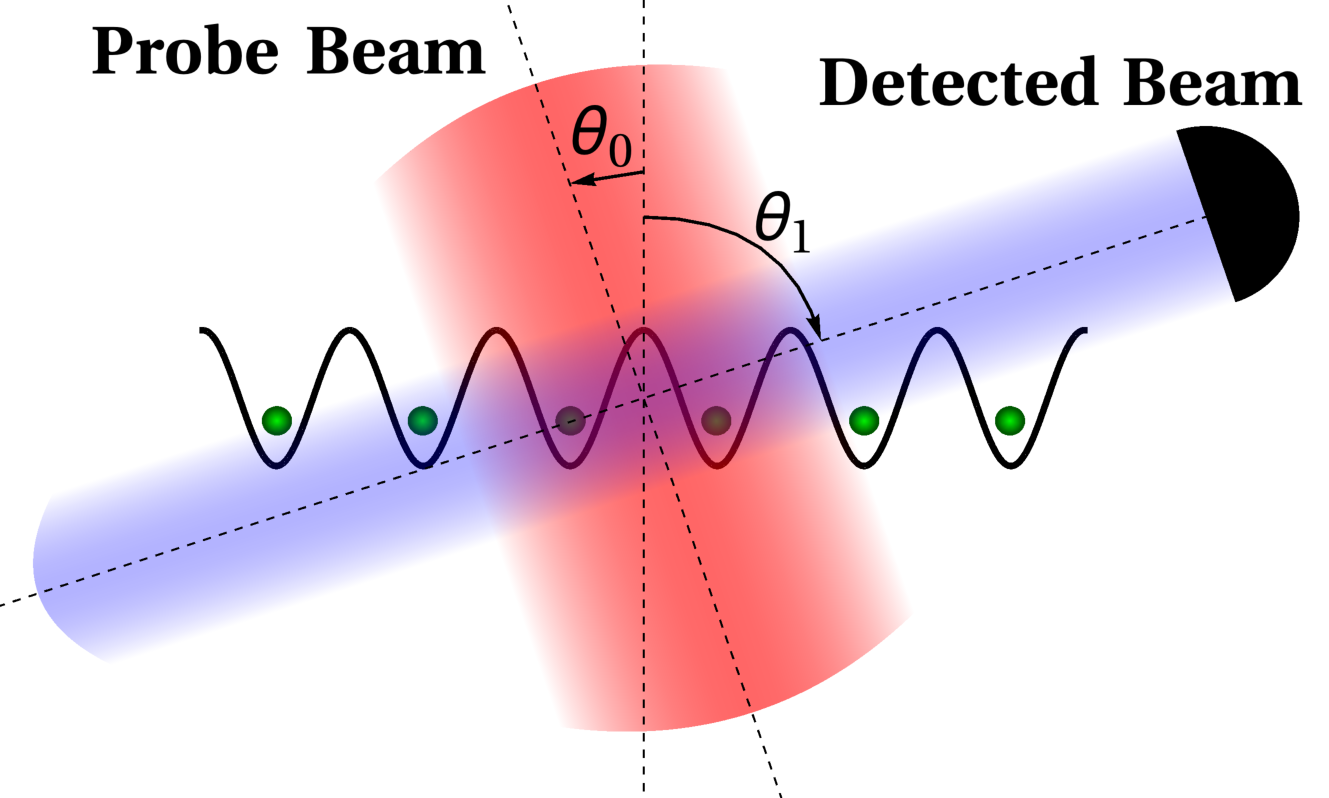
\includegraphics[width=1.0\textwidth]{LatticeDiagram}
  \caption[LatticeDiagram]{Atoms (green) trapped in an optical lattice
    are illuminated by a coherent probe beam (red). The light scatters
    (blue) in free space or into a cavity and is measured by a
    detector. If the experiment is in free space light can scatter in
    any direction. A cavity on the other hand enhances scattering in
    one particular direction.}
  \label{fig:LatticeDiagram}
\end{figure}

For simplicity, we will be considering one-dimensional lattices most
of the time. However, the model itself is derived for any number of
dimensions and since none of our arguments will ever rely on
dimensionality our results straightforwardly generalise to 2- and 3-D
systems. This simplification allows us to present a much simpler
picture of the physical setup where we only need to concern ourselves
with a single angle for each optical mode. As shown in
Fig. \ref{fig:LatticeDiagram} the angle between the normal to the
lattice and the probe and detected beam are denoted by $\theta_0$ and
$\theta_1$ respectively. We will consider these angles to be tunable
although the same effect can be achieved by varying the wavelength of
the light modes. However, it is much more intuitive to consider
variable angles in our model as this lends itself to a simpler
geometrical representation.

\subsection{Derivation of the Hamiltonian}

A general many-body Hamiltonian coupled to a quantized light field in
second quantized can be separated into three parts,
\begin{equation}
\label{eq:FullH}
  \H = \H_f + \H_a + \H_{fa}.
\end{equation}
The term $\H_f$ represents the optical part of the Hamiltonian,
\begin{equation}
\label{eq:Hf}
  \H_f = \sum_l \hbar \omega_l \ad_l \a_l -
  i \hbar \sum_l \left( \eta_l^* \a_l - \eta_l \ad \right).
\end{equation}
The operators $\a_l$ ($\ad$) are the annihilation (creation) operators
of light modes with frequencies $\omega_l$, wave vectors $\b{k}_l$,
and mode functions $u_l(\b{r})$, which can be pumped by coherent
fields with amplitudes $\eta_l$. The second part of the Hamiltonian,
$\H_a$, is the matter-field component given by
\begin{equation}
\label{eq:Ha}
  \H_a = \int \mathrm{d}^3 \b{r} \Psi^\dagger(\b{r}) \H_{1,a}
  \Psi(\b{r}) + \frac{2 \pi a_s \hbar^2}{m} \int \mathrm{d}^3 \b{r}
  \Psi^\dagger(\b{r}) \Psi^\dagger(\b{r}) \Psi(\b{r}) \Psi(\b{r}).
\end{equation}
Here, $\Psi(\b{r})$ ($\Psi^\dagger(\b{r})$) are the matter-field
operators that annihilate (create) an atom at position $\b{r}$, $a_s$
is the $s$-wave scattering length characterising the interatomic
interaction, and $\H_{1,a}$ is the atomic part of the single-particle
Hamiltonian $\H_1$. The final component of the total Hamiltonian is
the interaction given by 
\begin{equation}
  \label{eq:Hfa}
  \H_{fa} = \int \mathrm{d}^3 \b{r} \Psi^\dagger(\b{r}) \H_{1,fa}
  \Psi(\b{r}),
\end{equation}
where $\H_{1,fa}$ is the interaction part of the single-particle
Hamiltonian, $\H_1$.

The single-particle Hamiltonian in the rotating-wave and dipole
approximation is given by
\begin{equation}
  \H_1 = \H_f + \H_{1,a} + \H_{1,fa},
\end{equation}
\begin{equation}
  \H_{1,a} = \frac{\b{p}^2} {2 m_a} + \frac{\hbar \omega_a}{2} \sigma_z,
\end{equation}
\begin{equation}
  \H_{1,fa} =  - i \hbar \sum_l \left[ \sigma^+ g_l \a_l u_l(\b{r}) - \sigma^- g^*_l
    \ad_l u^*_l(\b{r}) \right].
\end{equation}
In the equations above, $\b{p}$ and $\b{r}$ are the momentum and
position operators of an atom of mass $m_a$ and resonance frequency
$\omega_a$. The operators $\sigma^+ = |g \rangle \langle e|$,
$\sigma^- = |e \rangle \langle g|$, and
$\sigma_z = |e \rangle \langle e| - |g \rangle \langle g|$ are the
atomic raising, lowering and population difference operators, where
$|g \rangle$ and $| e \rangle$ denote the ground and excited states of
the two-level atom respectively. $g_l$ are the atom-light coupling
constants for each mode. It is the inclusion of the interaction of the
boson with quantized light that distinguishes our work from the
typical approach to ultracold atoms where all the optical fields,
including the trapping potentials, are treated classically.

We will now simplify the single-particle Hamiltonian by adiabatically
eliminating the upper excited level of the atom. The equations of
motion for the time evolution of operator $\hat{A}$ in the Heisenberg
picture are given by
\begin{equation}
  \dot{\hat{A}} = \frac{i}{\hbar} \left[\H, \hat{A} \right].
\end{equation}
Therefore, the Heisenberg equation for the lowering operator of a
single particle is
\begin{equation}
  \dot{\sigma}^- = \frac{i}{\hbar} \left[\H_1, \hat{\sigma}^- \right]
  = \hbar \omega_a \sigma^- + i \hbar \sum_l \sigma_z g_l \a_l u_l(\b{r}).
\end{equation}
We will consider nonresonant interactions between light and atoms
where the detunings between the light fields and the atomic resonance,
$\Delta_{la} = \omega_l - \omega_a$, are much larger than the
spontaneous emission rate and Rabi frequencies $g_l \a_l$. Therefore,
the atom will be predominantly found in the ground state and we can
set $\sigma_z = -1$ which is also known as the linear dipole
approximation as the dipoles respond linearly to the light amplitude
when the excited state has negligible population. Moreover, we can
adiabatically eliminate the polarization $\sigma^-$. Firstly we will
re-write its equation of motion in a frame rotating at $\omega_p$, the
external probe frequency, such that
$\sigma^- = \tilde{\sigma}^- \exp(i \omega_p t)$, and similarly for
$\tilde{\a}_l$. The resulting equation is given by
\begin{equation}
  \dot{\tilde{\sigma}}^- = - \hbar \Delta_a \tilde{\sigma}^- - i \hbar
  \sum_l g_l \tilde{\a}_l u_l(\b{r}),
\end{equation}
where $\Delta_a = \omega_p - \omega_a$ is the atom-probe
detuning. Within this rotating frame we will take
$\dot{\tilde{\sigma}}^- \approx 0$ and thus obtain the following
equation for the lowering operator
\begin{equation}
  \sigma^- = - \frac{i}{\Delta_a} \sum_l g_l \a_l u_l(\b{r}).
\end{equation}
Therefore, by inserting this expression into the Heisenberg equation
for the light mode $m$ given by
\begin{equation}
  \dot{\a}_m = - \sigma^- g^*_m u^*_m(\b{r})
\end{equation}
we get the following equation of motion
\begin{equation}
  \dot{\a}_m = \frac{i}{\Delta_a} \sum_l g_l g^*_m u_l(\b{r})
  u^*_m(\b{r}) \a_l.
\end{equation}
An effective Hamiltonian which results in the same optical equations
of motion can be written as
$\H^\mathrm{eff}_1 = \H_f + \H^\mathrm{eff}_{1,a} +
\H^\mathrm{eff}_{1,fa}$. The effective atomic and interaction
Hamiltonians  are
\begin{equation}
\label{eq:aeff}
  \H^\mathrm{eff}_{1,a} = \frac{\b{p}^2}{2 m_a} + V_\mathrm{cl}(\b{r}),
\end{equation}
\begin{equation}
\label{eq:faeff}
  \H^\mathrm{eff}_{1,fa} = \frac{\hbar}{\Delta_a} \sum_{l,m}
  u_l^*(\b{r}) u_m(\b{r}) g_l g_m \ad_l \a_m,
\end{equation}
where we have explicitly extracted
$V_\mathrm{cl}(\b{r}) = \hbar g_\mathrm{cl}^2 |a_\mathrm{cl}
u_\mathrm{cl}(\b{r})|^2 / \Delta_{\mathrm{cl},a}$, the classical
trapping potential, from the interaction terms. However, we consider
the trapping beam to be sufficiently detuned from the other light
modes that we can neglect any scattering between them. A later
inclusion of this scattered light would not be difficult due to the
linearity of the dipoles we assumed.

Normally we will consider scattering of modes $a_l$ much weaker than
the field forming the lattice potential $V_\mathrm{cl}(\b{r})$. We now
proceed in the same way as when deriving the conventional Bose-Hubbard
Hamiltonian in the zero temperature limit. The field operators
$\Psi(\b{r})$ can be expanded using localised Wannier functions of
$V_\mathrm{cl}(\b{r})$ and by keeping only the lowest vibrational
state we get
\begin{equation}
  \Psi(\b{r}) = \sum_i^M b_i w(\b{r} - \b{r}_i),
\end{equation} 
where $b_i$ ($\bd_i$) is the annihilation (creation) operator of an
atom at site $i$ with coordinate $\b{r}_i$ and $M$ is the number of
lattice sites. Substituting this expression in Eq. \eqref{eq:FullH}
with $\H_{1,a} = \H_{1,a}^\mathrm{eff}$ and
$\H_{1,fa} = \H_{1,fa}^\mathrm{eff}$ given by Eq. \eqref{eq:aeff} and
\eqref{eq:faeff} respectively yields the following generalised
Bose-Hubbard Hamiltonian, $\H = \H_f + \H_a + \H_{fa}$, 
\begin{equation}
  \H = \H_f + \sum_{i,j}^M J^\mathrm{cl}_{i,j} \bd_i b_j + 
  \sum_{i,j,k,l}^M \frac{U_{ijkl}}{2} \bd_i \bd_j b_k b_l + 
  \frac{\hbar}{\Delta_a} \sum_{l,m} g_l g_m \ad_l \a_m 
  \left( \sum_{i,j}^K J^{l,m}_{i,j} \bd_i b_j \right).
\end{equation}
The optical field part of the Hamiltonian, $\H_f$, has remained
unaffected by all our approximations and is given by
Eq. \eqref{eq:Hf}. The matter-field Hamiltonian is now given by the
well known Bose-Hubbard Hamiltonian
\begin{equation}
  \H_a = \sum_{i,j}^M J^\mathrm{cl}_{i,j} \bd_i b_j + 
  \sum_{i,j,k,l}^M \frac{U_{ijkl}}{2} \bd_i \bd_j b_k b_l,
\end{equation}
where the first term represents atoms tunnelling between sites with a
hopping rate given by
\begin{equation}
  J^\mathrm{cl}_{i,j} = \int \mathrm{d}^3 \b{r} w (\b{r} - \b{r}_i ) 
  \left( -\frac{\b{p}^2}{2 m_a} + V_\mathrm{cl}(\b{r}) \right) w(\b{r}
  - \b{r}_i),
\end{equation}
and $U_{ijkl}$ is the interaction strength given by
\begin{equation}
  U_{ijkl} = \frac{4 \pi a_s \hbar^2}{m_a} \int \mathrm{d}^3 \b{r} 
  w(\b{r} - \b{r}_i) w(\b{r} - \b{r}_j) w(\b{r} - \b{r}_k) w(\b{r} - \b{r}_l).
\end{equation}
